\documentclass[border=6pt]{standalone}
\usepackage[T1]{fontenc}\usepackage{lmodern}\usepackage{amsmath,amssymb}\usepackage{graphicx}\usepackage{xcolor}\usepackage{tikz}
\usetikzlibrary{arrows.meta,positioning,calc,fit,shapes.misc,shapes.geometric}
% TikZ styles
\tikzset{
  blk/.style={draw, rounded corners=2pt, align=center, font=\small, minimum height=8mm, inner sep=4pt, fill=#1},
  blk/.default=white,
  arr/.style={-{Stealth[length=2.2mm]}, thick},
}
\definecolor{base}{HTML}{FBE3E3}
\definecolor{prop}{HTML}{DDEBFA}
\definecolor{same}{HTML}{EDEDED}
\definecolor{done}{HTML}{DFF1DF}
\definecolor{todo}{HTML}{FFF2CC}

\begin{document}
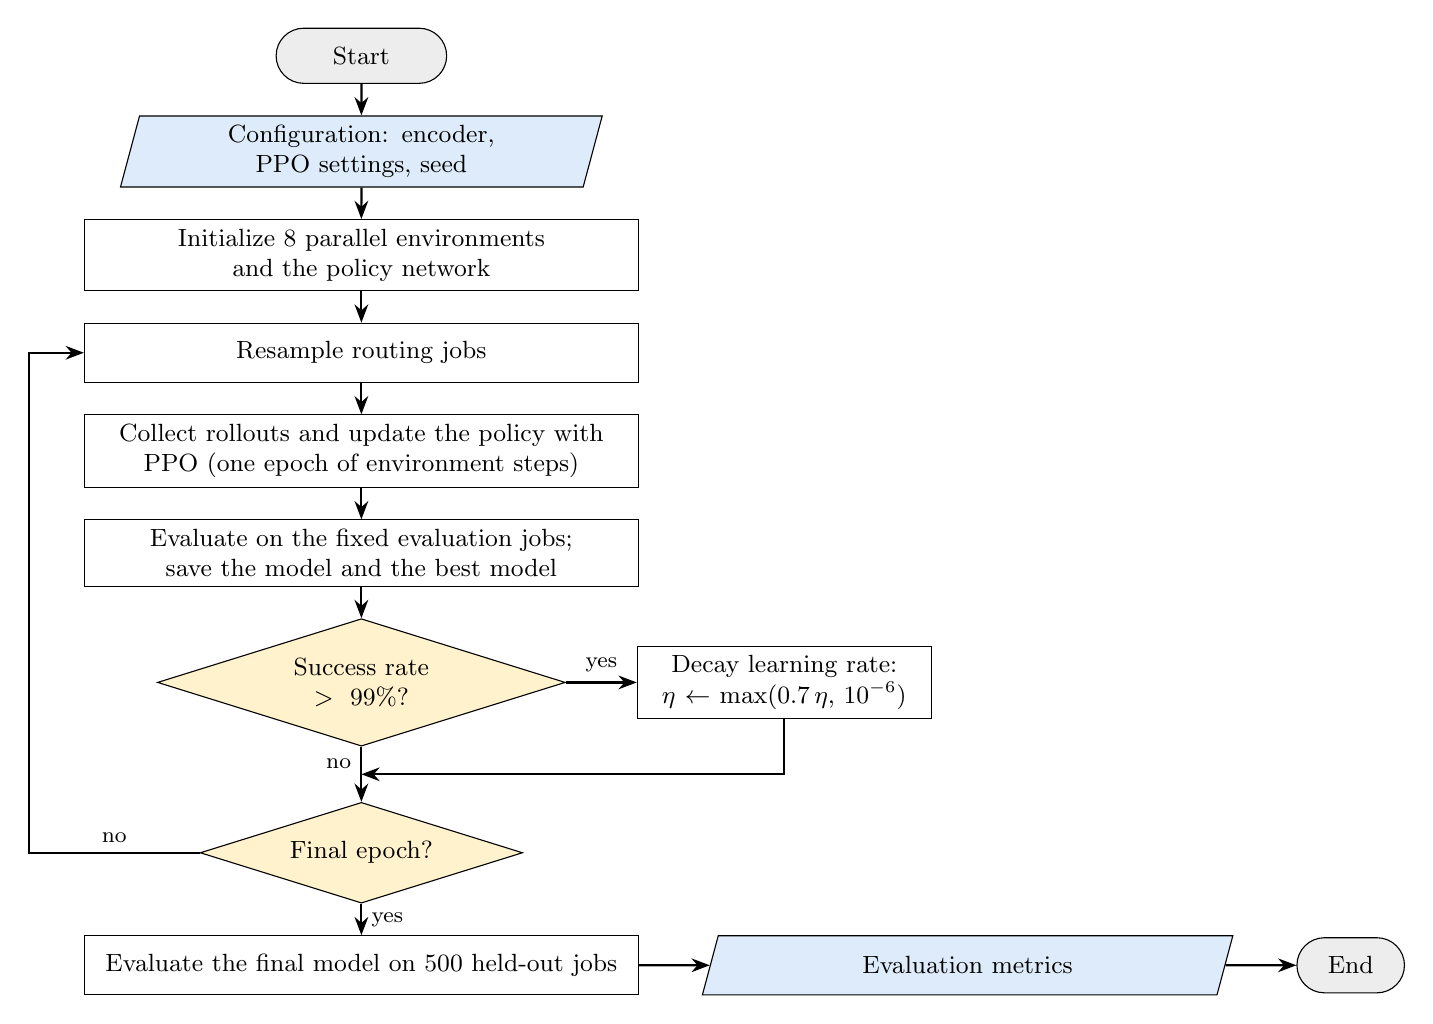
\begin{tikzpicture}[>=Stealth, font=\small, node distance=4mm,
  term/.style={draw, rounded rectangle, fill=same, minimum height=7mm, minimum width=2.4cm},
  proc/.style={draw, rectangle, fill=white, minimum height=7.5mm, text width=6.8cm, align=center,
    execute at begin node={\hyphenpenalty=10000\relax}},
  data/.style={draw, trapezium, trapezium left angle=75, trapezium right angle=105, fill=prop, minimum height=7.5mm, text width=5.4cm, align=center},
  dec/.style={draw, diamond, aspect=3.2, fill=todo, inner sep=1pt, align=center, text width=2.9cm},
  flow/.style={->, thick}]
  \node[term] (start) {Start};
  \node[data, below=of start] (cfg) {Configuration: encoder, PPO settings, seed};
  \node[proc, below=of cfg] (init) {Initialize 8 parallel environments\\ and the policy network};
  \node[proc, below=of init] (jobs) {Resample routing jobs};
  \node[proc, below=of jobs] (train) {Collect rollouts and update the policy with\\ PPO (one epoch of environment steps)};
  \node[proc, below=of train] (eval) {Evaluate on the fixed evaluation jobs;\\ save the model and the best model};
  \node[dec, below=of eval] (d1) {Success rate $>99\%$?};
  \node[proc, right=9mm of d1, text width=3.5cm] (lr) {Decay learning rate:\\ $\eta\leftarrow\max(0.7\,\eta,\,10^{-6})$};
  \node[dec, below=7mm of d1] (d2) {Final epoch?};
  \node[proc, below=of d2] (final) {Evaluate the final model on 500 held-out jobs};
  \node[data, right=9mm of final, text width=3.6cm] (out) {Evaluation metrics};
  \node[term, right=9mm of out, minimum width=1.6cm] (stop) {End};
  \draw[flow] (start) -- (cfg);
  \draw[flow] (cfg) -- (init);
  \draw[flow] (init) -- (jobs);
  \draw[flow] (jobs) -- (train);
  \draw[flow] (train) -- (eval);
  \draw[flow] (eval) -- (d1);
  \draw[flow] (d1) -- node[above, font=\footnotesize] {yes} (lr);
  \draw[flow] (d1) -- node[left, pos=0.3, font=\footnotesize] {no} (d2);
  \coordinate (join) at ($(d1.south)!0.5!(d2.north)$);
  \draw[flow] (lr.south) |- (join);
  \draw[flow] (d2) -- node[right, font=\footnotesize] {yes} (final);
  \draw[flow] (d2.west) -| node[above, pos=0.25, font=\footnotesize] {no} ([xshift=-7mm]jobs.west) -- (jobs.west);
  \draw[flow] (final) -- (out);
  \draw[flow] (out) -- (stop);
\end{tikzpicture}
\end{document}
